\chapter{Real-Life Measurements}

\section{Introduction}

idkmybffjill

\section{Needle Probe Measurement Fundamentals}

Needle probe measurements were taken using an apparatus borrowed from the Cold
Regions Research and Engineering Laboratory, illustrated in figure
\ref{fig:apparatus}. Encased in a Pelican case for protection are a Campbell
CR10X data logger, a relay switch, a 12v gel cell for the CR10X and a series of
D-cells to power the heating coils in the needle. The program that came with the
data logger uses the relay switch to control the heat flux from the needle, and
records temperature data from the needle's thermocouple, as well as the voltage
across the heating element, over the course of a five minute heating curve and
a ten minute cooling curve.

\begin{figure}[h]
\centering
\includegraphics[width=0.7\textwidth]{fig/apparatus.png}
\label{fig:apparatus}
\caption{Extruded illustration of the needle probe apparatus. Major parts are labelled.}
\end{figure}

The apparatus is controlled using a keypad that enables one to communicate
with the data logger using Campbell ``star-codes.'' Initiating a test is a
matter of clearing and setting some registers using these star-codes.

\marginpar{source star codes?}

In general, the apparatus is used like so:

\begin{enumerate}
\item Turn on device.
\item Insert needle into medium being measured.
\item Use star-codes to clear the first three registers. ``* 6 A'' accesses the
registers, and ``D <n>'' toggles the nth register. For example, to clear
the second register, press ``* 6 A D 2'' .
\item Turn on the first register by pressing ``* 6 A D 1''. This makes the
apparatus measure temperature.
\item Turn on the second register by pressing ``* 6 A D 2''. This turns on the
heating element, effectively starting the test.
\item Wait 15 minutes for test to complete.
\end{enumerate}

Once testing is complete, data may be uploaded from the data logger using
Campbell's PC200X software and a particular series of cables and devices, as
shown in figure \ref{fig:cable}. In order, from datalogger to computer, they
are:

\marginpar{Source PC200X?}

\begin{enumerate}
\item A DE-9 cable
\item an SC32A optically isolating RS-232 interface
\item A DB-25-to-DE-9 serial cable
\item A DE-9 Null Modem cable
\item (Optional) A DE-9-to-USB cable
\end{enumerate}

Given the correct cables and ports, one may be able to decrease the number of
cables to two, plus the SC32A interface.

\begin{figure}[h]
\centering
\includegraphics[width=0.6\textwidth]{fig/cable.jpg}
\label{fig:cable}
\caption{The cables used to communicate with the datalogger.}
\end{figure}




\section{Snow Conductivity Measurements}
\begin{figure}[h]
\centering
\includegraphics[width=0.8\textwidth]{fig/equipment.jpg}
\label{fig:equipment}
\caption{Equipment used to measure snow thermal conductivity.}
\end{figure}

\begin{figure}[h]
\centering
\includegraphics[width=0.4\textwidth]{fig/insitu_location.jpg}
\label{fig:insitu_location}
\caption{The location for in-situ tests.}
\end{figure}

\begin{figure}[h]
\centering
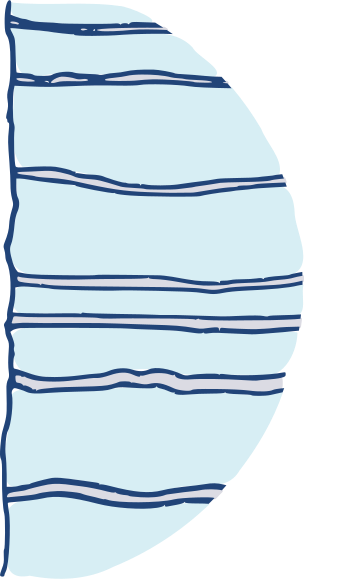
\includegraphics[width=0.8\textwidth]{fig/snowpack.jpg}
\label{fig:snowpack}
\caption{A close-up shot of tested snowpack.}
\end{figure}

The data

The analysis

\section{Benchtop Tests with Glycerine}

The box

\section{Anisotropic Glycerine}

Layers

low K layer

high K layer

tests of both materials alone

\section{Snow Measurements}

technique
